\documentclass[11pt]{article}

\usepackage[a4paper,margin=26mm]{geometry}
\usepackage[T1]{fontenc}
\usepackage[utf8]{inputenc}
\usepackage{lmodern}
\usepackage{microtype}
\usepackage{amsmath,amssymb,amsthm,mathtools}
\usepackage{xcolor}
\usepackage{enumitem}
\usepackage{hyperref}
\usepackage{tikz}
\usepackage[most]{tcolorbox}
\usetikzlibrary{calc}

\definecolor{boxblue}{RGB}{235,244,252}
\definecolor{boxgreen}{RGB}{237,248,241}
\definecolor{boxgray}{RGB}{246,246,246}
\definecolor{darkblue}{RGB}{25,75,120}

\hypersetup{
  colorlinks=true,
  linkcolor=darkblue,
  urlcolor=darkblue,
  pdftitle={A Cyclic Hub Obstruction for Monohedral Tilings of a Disk}
}

\newtheorem{theorem}{Theorem}
\newtheorem{proposition}[theorem]{Proposition}
\newtheorem{lemma}[theorem]{Lemma}
\theoremstyle{definition}
\newtheorem{definition}[theorem]{Definition}
\theoremstyle{remark}
\newtheorem{remark}[theorem]{Remark}

\newcommand{\D}{D}
\newcommand{\T}{T}
\newcommand{\Kreg}{\mathcal K}

\newtcolorbox{plainbox}[1][boxgray]{
  colback=#1,
  colframe=#1,
  boxrule=0pt,
  arc=1.5mm,
  left=3mm,right=3mm,top=2.5mm,bottom=2.5mm,
  before skip=7pt,after skip=7pt
}

\title{\textbf{A Cyclic Hub Obstruction for Monohedral Tilings of a Disk}\\[2mm]
\large A short note on one-ring and multi-ring rotational contact structures}
\author{Research note}
\date{August 2026}

\begin{document}
\maketitle

\begin{abstract}
We record a simple obstruction for rotationally symmetric monohedral tilings of a Euclidean disk.  A tile fixed by a rotation cannot have its whole boundary covered by one cyclic orbit of connected interfaces with congruent neighbouring tiles.  The proof uses only periodicity of the signed curvature along the fixed tile and cancellation of curvature across internal interfaces.  Consequently, adding any number of outer rings does not remove the obstruction.  We also give the corresponding abelianized word certificate, which is suitable for formal contour-matching algorithms.
\end{abstract}

\begin{plainbox}[boxblue]
\textbf{Informal statement.}
A monohedral disk tiling cannot consist of a rotationally fixed central tile whose boundary is divided into $k$ equivalent connected contacts with one orbit of $k$ surrounding tiles.  Placing further rings outside those tiles does not help: the contradiction is already forced at the central tile.
\end{plainbox}

\section{Setting and hypotheses}

Let $\D\subset\mathbb R^2$ be a closed Euclidean disk.  A \emph{monohedral tiling} of $\D$ is a finite family of congruent Jordan regions
\[
  \D=\T_0\cup\T_1\cup\cdots\cup\T_{N-1}
\]
with pairwise disjoint interiors.  Throughout this note, every tile boundary is assumed to be piecewise $C^2$, with finitely many exceptional points.  Curvature integrals below are taken only over the $C^2$ portions; corner contributions are not included.

Assume that the tiling is preserved by a rotation $r$ of order $k\ge 2$ about the centre of $\D$.  We call $\T_0$ a \emph{cyclic hub} if
\[
  r(\T_0)=\T_0
\]
and if there is one orbit of distinct neighbouring tiles
\[
  \T_1,\ldots,\T_k,\qquad r(\T_i)=\T_{i+1}\quad (\bmod k),
\]
such that the following conditions hold.

\begin{enumerate}[label=(H\arabic*),leftmargin=12mm]
\item Each intersection
\[
  C_i=\partial\T_0\cap\partial\T_i
\]
is a single non-degenerate connected boundary arc.
\item The arcs $C_1,\ldots,C_k$ have pairwise disjoint relative interiors and cover the hub boundary:
\[
  \partial\T_0=C_1\cup\cdots\cup C_k.
\]
\item No other tile has a positive-length contact with $\T_0$.
\end{enumerate}

The positive-length contact graph therefore has a fixed vertex $\T_0$ whose incident edges form exactly one orbit of size $k$.  No assumption is made about contacts among the $\T_i$, nor about tiles farther from the hub.

\begin{center}
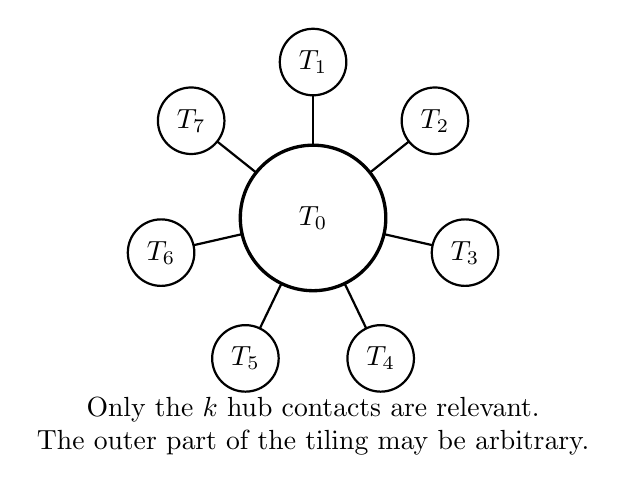
\begin{tikzpicture}[scale=0.88]
  \def\k{7}
  \draw[very thick] (0,0) circle (1.05);
  \node at (0,0) {$\T_0$};
  \foreach \i in {0,...,6}{
    \coordinate (P\i) at ({90-360/7*\i}:2.25);
    \draw[thick] (P\i) circle (0.48);
    \node at (P\i) {$\T_{\number\numexpr\i+1\relax}$};
    \draw[thick] ({90-360/7*\i}:1.05) -- ({90-360/7*\i}:1.77);
  }
  \node[align=center] at (0,-3.0) {Only the $k$ hub contacts are relevant.\\The outer part of the tiling may be arbitrary.};
\end{tikzpicture}
\end{center}

\section{The two obstruction theorems}

\begin{theorem}[One-ring cyclic hub obstruction]\label{thm:one-ring}
There is no rotationally symmetric monohedral tiling of a Euclidean disk satisfying \emph{(H1)--(H3)}.  Equivalently, a fixed central tile cannot have its entire boundary divided into one $C_k$-orbit of $k$ connected interfaces with one orbit of $k$ neighbouring congruent tiles.
\end{theorem}

\begin{plainbox}[boxgreen]
\textbf{Intuitive version of Theorem~\ref{thm:one-ring}.}
The rotation makes the contour of the central tile periodic, with one period equal to one central contact.  The same physical contact, viewed from the neighbouring tile, must have the opposite signed bending.  But on the common prototype it is another arc of exactly one period, so periodicity gives it the same signed bending.  Hence one period has zero signed bending.  All congruent tiles then have zero regular signed bending, while the outer circle contributes $2\pi$.  This is impossible.
\end{plainbox}

\begin{theorem}[Outer rings do not help]\label{thm:many-rings}
Assume a rotationally symmetric monohedral tiling contains a cyclic hub satisfying \emph{(H1)--(H3)}.  Then the tiling is impossible, regardless of how many further tile orbits or ``rings'' occur outside the first neighbour orbit, and regardless of the positive-length contacts among those outer tiles.
\end{theorem}

\begin{plainbox}[boxblue]
\textbf{What ``several rings'' means here.}
The theorem does \emph{not} require consecutive rings to be cycles, to touch by one edge orbit, or even to admit a clean annular decomposition.  The outer contact graph may be arbitrary.  The only decisive condition is local to the hub: one orbit of $k$ neighbours, one connected hub interface per neighbour, and those $k$ interfaces covering all of $\partial\T_0$.
\end{plainbox}

Theorem~\ref{thm:many-rings} is an immediate consequence of Theorem~\ref{thm:one-ring}, but it is stated separately because it is the form most useful when enumerating layered contact maps.

\section{Signed curvature bookkeeping}

For a positively oriented piecewise $C^2$ Jordan curve $\Gamma$, define its \emph{regular signed curvature}
\[
  \Kreg(\Gamma)=\int_{\Gamma_{\mathrm{reg}}}\kappa\,ds,
\]
where the finitely many non-$C^2$ points are omitted.  The same notation is used for a boundary subarc.

\begin{lemma}[Cancellation identity]\label{lem:cancellation}
For any finite tiling of the disk by piecewise $C^2$ Jordan regions,
\[
  \sum_{j=0}^{N-1}\Kreg(\partial\T_j)=2\pi.
\]
\end{lemma}

\begin{proof}
Give every tile boundary its positive orientation.  Every regular internal interface is traversed in opposite directions by the two incident tiles, so its two signed curvature integrals cancel.  After all internal interfaces have cancelled, only the boundary of the ambient disk remains.  That boundary is a positively oriented circle and contributes $2\pi$.
\end{proof}

\begin{lemma}[One-period curvature]\label{lem:period}
Let $P$ be a piecewise $C^2$ Jordan region invariant under a rotation of order $k$.  Let $L=\operatorname{per}(P)/k$.  Then every positively oriented boundary interval of arclength $L$ has the same regular signed curvature.
\end{lemma}

\begin{proof}
The rotation acts freely on $\partial P$ and preserves arclength and the positive boundary orientation.  In arclength coordinates, the regular curvature density is therefore $L$-periodic.  The integral of an $L$-periodic integrable function over any interval of length $L$ is independent of the starting point.
\end{proof}

\section{Proof of the obstruction}

\begin{proof}[Proof of Theorem~\ref{thm:one-ring}]
Use $P=\T_0$ as the prototype.  Since the $k$ hub interfaces are permuted transitively by the rotation and cover $\partial\T_0$, each has arclength
\[
  L=\frac{\operatorname{per}(P)}{k}.
\]
Let
\[
  K=\Kreg(C_1).
\]
By rotational symmetry, every $C_i$ has the same regular signed curvature $K$, and hence
\[
  \Kreg(\partial P)=kK. \tag{1}
\]

Now consider the same physical interface $C_1$ as part of the positively oriented boundary of the neighbouring tile $\T_1$.  Because the two tiles lie on opposite sides of the interface, the two positive boundary orientations traverse the regular part of $C_1$ in opposite directions.  Therefore its curvature contribution on $\T_1$ is
\[
  -K. \tag{2}
\]

Transport this boundary arc of $\T_1$ back to the common prototype $P$ by any congruence.  When an indirect congruence is used, reflection and reversal of the boundary orientation compensate; thus regular signed curvature in the positive boundary orientation is preserved.  We obtain a boundary interval $J\subset\partial P$ of arclength $L$ satisfying
\[
  \Kreg(J)=-K. \tag{3}
\]

By Lemma~\ref{lem:period}, every boundary interval of $P$ having arclength $L$ has curvature $K$.  In particular,
\[
  \Kreg(J)=K. \tag{4}
\]
Combining (3) and (4) gives
\[
  K=0.
\]
Equation (1) then yields
\[
  \Kreg(\partial P)=0.
\]
All tiles are congruent to $P$, so every tile has zero regular signed curvature.  Consequently
\[
  \sum_{j=0}^{N-1}\Kreg(\partial\T_j)=0,
\]
contradicting Lemma~\ref{lem:cancellation}.  Hence the tiling cannot exist.
\end{proof}

\begin{proof}[Proof of Theorem~\ref{thm:many-rings}]
The proof of Theorem~\ref{thm:one-ring} uses only the fixed hub $\T_0$, its first orbit of $k$ neighbours, and the global cancellation identity.  No adjacency or geometric information concerning the remaining tiles enters the argument.  Therefore arbitrary additional outer rings or contact structures cannot remove the contradiction.
\end{proof}

\section{Formal word certificate}

The same obstruction appears before coordinates are introduced.

Let $\mathcal A$ be an alphabet of signed contour atoms, equipped with a duality $a\mapsto a^*$ corresponding to viewing the same interface from the opposite tile.  Let
\[
  q:\mathbb Z^{(\mathcal A)}\longrightarrow G
\]
be an additive charge into a torsion-free abelian group, invariant under the allowed mirror/reversal operators and satisfying
\[
  q(a^*)=-q(a).
\]
For example, $q$ may record signed curvature classes or signed circular-arc types.

\begin{proposition}[Abelianized certificate]\label{prop:word}
Suppose the cyclic prototype word has the form
\[
  W=U^k,
\]
a hub interface uses the period word $U$, and its partner on the neighbouring copy is a cyclic factor $V$ of $W$ with $|V|=|U|$.  If the interface equation gives
\[
  q(V)=-q(U),
\]
then
\[
  q(U)=q(W)=0.
\]
Hence no exact tiling can realize this word system whenever cancellation of internal interfaces leaves a non-zero exterior charge.
\end{proposition}

\begin{proof}
Every cyclic factor of $U^k$ having length $|U|$ is a cyclic conjugate of $U$, so it has the same abelianization and therefore
\[
  q(V)=q(U).
\]
Together with $q(V)=-q(U)$ this gives $2q(U)=0$.  Since $G$ is torsion-free, $q(U)=0$, and then $q(W)=kq(U)=0$.  Summing the charge over all copies cancels every internal interface.  If the remaining exterior boundary has non-zero charge, a contradiction follows.
\end{proof}

\begin{plainbox}[boxgreen]
\textbf{Algorithmic reading.}
After quotienting atom names by the $C_k$ action on the central tile, the central contour is a power $U^k$.  The partner of $U$ is another length-$|U|$ factor of the same cyclic word, so it has the same abelianized inventory.  Interface duality requires the opposite signed inventory.  This gives a tiny unsatisfiable core, before lengths, angles, coordinates, or weak-order refinement are solved.
\end{plainbox}

\section{Scope and escape routes}

The obstruction is intentionally precise.  It does not directly cover the following situations.

\begin{enumerate}[leftmargin=8mm]
\item \textbf{More than one neighbour orbit at the hub.}  A fundamental sector of $\partial\T_0$ may be split among two or more tile orbits.  An individual interface then has length smaller than one full period, so Lemma~\ref{lem:period} no longer compares it with every possible partner arc.

\item \textbf{Disconnected hub contacts.}  The contact $\partial\T_0\cap\partial\T_i$ may have several separated components.  Their transported partners need not form one boundary interval of length $\operatorname{per}(P)/k$.

\item \textbf{Purely combinatorial cyclic symmetry.}  An automorphism of the contact graph is not enough.  The proof requires a genuine geometric rotation, or equivalently an actual order-$k$ periodic action on the contour of the fixed tile.

\item \textbf{Very irregular boundaries.}  The present proof is stated for piecewise $C^2$ boundaries.  A formulation using curvature measures for curves of finite total curvature should extend the result, but is not developed here.
\end{enumerate}

Thus a rotationally fixed tile can only survive by breaking the one-orbit, one-connected-contact hub structure.  In a formal search, the first alternatives to test are therefore multiple tile orbits meeting the hub within each fundamental sector, or disconnected central interfaces.

\section*{Conclusion}

The obstruction may be summarized in contact-graph language as follows:

\begin{plainbox}[boxblue]
If a rotationally fixed tile has degree $k$, its $k$ positive-length incident contacts form one $C_k$-orbit, each contact is connected, and these contacts cover the whole tile boundary, then no monohedral tiling of a Euclidean disk exists.  This remains true after attaching an arbitrary contact structure outside the first neighbour orbit.
\end{plainbox}

\end{document}
